\documentclass[a4paper, 10pt]{report}

% metadata
% ---------------------------------------------------------------------------

\newcommand{\name}{Naoki Pross}
\newcommand{\instructor}{Rinaldo Geiler, Daniele Kamm}
\newcommand{\specialization}{S.2 Sviluppare prototipi}

\newcommand{\project}{Spectrum Analyzer}
\newcommand{\projstart}{12.04.2018}
\newcommand{\projend}{15.05.2018}
\newcommand{\projectyear}{2017-18}

\newcommand{\plannedtime}{83 UD}
\newcommand{\actualtime}{-- UD}

% ---------------------------------------------------------------------------
% layout
\usepackage[
    inner=3cm,
    outer=3cm,
    top=3.5cm,
    bottom=3.5cm
]{geometry}

\usepackage{fancyhdr}
\pagestyle{fancy}
\fancyhf{}
\fancyhead[L]{CAM-SAM}
\fancyhead[C]{Elettronico}
\fancyhead[R]{\today}
\fancyfoot[L]{\jobname.tex}
\fancyfoot[C]{\name}
\fancyfoot[R]{\thepage}

\usepackage{afterpage}
\usepackage{titlesec}

\titleformat{\chapter}[hang]{\Huge\bfseries}
    {\thechapter}{.5em}{\thispagestyle{fancy}}
\titlespacing*{\chapter}{0pt}{-30pt}{10pt}

% language
\usepackage[italian]{babel}

% quotes
\usepackage{csquotes}
\usepackage{fancyvrb}

% sans serif font
\renewcommand{\familydefault}{\sfdefault}

% urls
\usepackage[
    colorlinks=true,
    linkcolor=.,
	citecolor=.,
    urlcolor=blue
]{hyperref}

% maths
\usepackage{amsmath}
\usepackage{amssymb}
\usepackage{amsthm}

% logo
\usepackage{metalogo}

% figures
\usepackage{float}
\usepackage{subfig}
% tables
\usepackage{array}
\usepackage{booktabs}
\usepackage{tabularx}
% plots
\usepackage{pgfplots}
\usepgfplotslibrary{fillbetween}
\pgfplotsset{compat=1.14}
% diagrams
\usepackage{tikz}
\usetikzlibrary{calc}
\usetikzlibrary{quotes}
\usetikzlibrary{patterns}
\usetikzlibrary{angles}
\usepackage[european]{circuitikz}
\usepackage{tikz-timing}
\usepackage{tikzscale}

% include PDFs
\usepackage{pdfpages}

% code
\usepackage{xcolor}
\usepackage{listings}

\lstdefinelanguage{diff}{
    sensitive=true,
    % diff command line
    morecomment=[f][\color{gray}][0]{diff},
    % commit identifiers for git diff
    morecomment=[f][\color{gray}][0]{index},
    % hunk location/line numbers for unified format
    morecomment=[f][\color{blue}][0]{@@},
    % hunk location/line numbers for context format
    morecomment=[f][\color{magenta}][0]{***},
    % changed line for context format
    morecomment=[f][\color{violet}][0]{!},
    % deleted lines for unified format
    morecomment=[f][\color{red!60!black}][0]-,
    % added lines for unified format
    morecomment=[f][\color{green!60!black}][0]+,
    % file name and time stamp old file
    morecomment=[f][\color{magenta}][0]{---},
    % file name and time stamp new file
    morecomment=[f][\color{magenta}][0]{+++},
    % Binary files ... differ
    morecomment=[f][\color{gray}][0]{Binary},
    % Only in ...: file.txt
    morecomment=[f][\color{gray}][0]{Only},
    % old mode ...
    morecomment=[f][\color{gray}][0]{old},
    % new mode ...
    morecomment=[f][\color{gray}][0]{new},
    % rename from/to ...
    morecomment=[f][\color{gray}][0]{rename},
    % similarity index ...%
    morecomment=[f][\color{gray}][0]{similarity},
    % deleted file mode ...%
    morecomment=[f][\color{gray}][0]{deleted},
    % hunk separator for context format
    morecomment=[f][\color{magenta}][0]{***************},
    % deleted lines for normal format
    morecomment=[f][\color{red!60!black}][0]<,
    % added lines for normal format
    morecomment=[f][\color{green!60!black}][0]>,
    % line number specifier for normal format
    morecomment=[f][\color{blue}][0]{0},
    % line number specifier for normal format
    morecomment=[f][\color{blue}][0]{1},
    % line number specifier for normal format
    morecomment=[f][\color{blue}][0]{2},
    % line number specifier for normal format
    morecomment=[f][\color{blue}][0]{3},
    % line number specifier for normal format
    morecomment=[f][\color{blue}][0]{4},
    % line number specifier for normal format
    morecomment=[f][\color{blue}][0]{5},
    % line number specifier for normal format
    morecomment=[f][\color{blue}][0]{6},
    % line number specifier for normal format
    morecomment=[f][\color{blue}][0]{7},
    % line number specifier for normal format
    morecomment=[f][\color{blue}][0]{8},
    % line number specifier for normal format
    morecomment=[f][\color{blue}][0]{9},
}[comments]

\lstdefinestyle{cc}{
    belowcaptionskip=1\baselineskip,
    breaklines=true,
    frame=none,
    % margin
    xleftmargin=\parindent,
    % numbers
    numbers=left,
    numbersep=5pt,
    numberstyle=\ttfamily\footnotesize\color{gray},
    %
    language=C,
    showstringspaces=false,
    % font
    basicstyle=\ttfamily\small,
    keywordstyle=\color{green!40!black},
    commentstyle=\color{gray},
    identifierstyle=\color{black},
    stringstyle=\color{orange},
}
\lstset{escapechar=`, style=cc}

\lstdefinestyle{smallcc}{
    belowcaptionskip=1\baselineskip,
    breaklines=true,
    frame=none,
    % margin
    xleftmargin=\parindent,
    % numbers
    numbers=left,
    numbersep=5pt,
    numberstyle=\ttfamily\footnotesize\color{gray},
    %
    language=C,
    showstringspaces=false,
    % font
    basicstyle=\ttfamily\small,
    keywordstyle=\color{green!40!black},
    commentstyle=\color{gray},
    identifierstyle=\color{black},
    stringstyle=\color{orange},
}

% ---------------------------------------------------------------------------
\newcommand{\dd}[1]{\mathrm{d}#1}

\newcommand\blankpage{%
    \null
    \thispagestyle{empty}%
    \addtocounter{page}{-1}%
    \newpage
}

% ---------------------------------------------------------------------------
\begin{document}

    \begin{titlepage}
\thispagestyle{empty}
\newgeometry{margin=3cm}
\renewcommand{\arraystretch}{1.5}

\begin{tikzpicture}[remember picture,overlay]
    \node[anchor=north west, inner sep=0pt] 
        at ($(current page.north west)+(3cm, -3cm)$) {
            \includegraphics[height=2.25cm]{figures/logo/LOGO_SAM}
        };
\end{tikzpicture}

\begin{flushright}
    \LARGE \bfseries
    Anno scolastico \projectyear \\
    Lavoro Professionale Individuale
\end{flushright}

\large
\begin{tabularx}{\textwidth}{l X}
    \midrule
    Nome Cognome: & \textbf{\name} \\

    \midrule
    Professione: & \textbf{Elettronico} \\

    \midrule
    Titolo del progetto: & \textbf{\project} \\

    \midrule
\end{tabularx}
\vfill

% immagine opizonale
% \includegraphics[\height=]{figures}

\vfill
\begin{tabularx}{\textwidth}{l X l X}
    \midrule
    Azienda: & \multicolumn{3}{l}{\parbox{5cm}{
        \textbf{CPT Bellinzona} \\
        Centro Professionale Tecnico \\
        Viale S. Franscini 25 \\
        6500 Bellinzona%
    }} \\

    \midrule
    Formazione approfondita: & \multicolumn{3}{l}{\textbf{\specialization}} \\

    \midrule
    Formatore: & \multicolumn{3}{l}{\textbf{\instructor}} \\

    \midrule
    Data d'inizio: & \textbf{\projstart} & Ore a disposizione: & \textbf{\plannedtime}\\

    \midrule
    Data file lavoro: & \textbf{\projend} & Ore effettive: &  \textbf{\actualtime} \\

    % \midrule
    % Data di compilazione & \textbf{\today} \\

    \midrule
\end{tabularx}

\restoregeometry
\end{titlepage}

    \blankpage
    \tableofcontents

	% spacing between paragraphs
	\setlength{\parskip}{.5em}

	\chapter{Introduzione}

\section{Contesto}
Per portare a termine il percorso formativo per un attestato di capacit\`a
federale presso la Scuola Arti e Mestieri di Bellinzona \`e richiesto lo
sviluppo individuale di un progetto di produzione di un prodotto.
Per interesse personale nella matematica della trasformata di Fourier mi \`e
stato assegnato di sviluppare un analizzatore spettrale.

\section{Requisiti}
\`E richiesto di sviluppare circuito per analizzare lo spettro dei segnali di
frequenza fino a 10\,kHz. Il dispositivo dovr\`a avere 3 possibili sorgenti:
RCA/Cinch e 2 Audio Jack per un microfono e per una sorgente di audio
generica. \`E inoltre richiesto che il calcolo dei dati dello spettrogramma
sia eseguito da un microcontroller della Microchip, collegato a due
altri dispositivi quali, una display e ad un computer in RS232, per poter
visualizzare lo spettrogramma computato.

\section{Concetto matematico}


\section{Norme di progetto}

	\chapter{Hardware}
\section{Schema a blocchi}

\section{Selezione delle entrate}
Essendo richiesta dai requisiti la possibilit\`a di selezione tra 3 entrate,
\`e stato utilizzando un semplice multiplexer controllato direttamente dal
microcontroller. Per la sua semplicit\`a non sono necessari particolari
osservarzioni.

\begin{figure}[H] \centering
    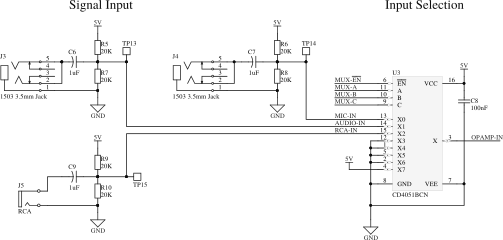
\includegraphics[width=.8\linewidth]{figures/circuits/input-selection.pdf}
    \caption{Circuito di selezione delle entrate \label{fig:input-selection}}
\end{figure}

Tutte le entrate dispongono di un condensatore di disaccoppiamento seguito da
un partitore di tensione simmetrico per aggiungere un offset della met\`a
dell'alimentazione. Il valore delle resistenze di 20\,k\(\Omega\) \`e scelto
per avere un impedenza rispetto al connettore pari all'impedenza
caratteristica dei cavi audio di 10\,k\(\Omega\).

\section{Circuito di entrata}
Il segnale di cui si analizza lo spettro, prima di essere campionato, viene
adattato mediate un circuito di amplificazione e filtraggio. Esso \`e
necessario per due ragioni. Il circuito di amplificazione \`e presente per
ovvie ragioni, quali per poter adattare il circuito nel caso in cui si dovesse
avere in entrata un segnale di ampiezza molto piccola. Il secondo circuito
invece, di filtraggio, \`e necessario per rimuovere disturbi di alta frequenza
che potrebbero compromettere la qualit\`a del campionamento. Questa \`e una
tipica configurazione prima di un circuito di conversione AD (analogico -
digitale), ed \`e conosciuto anche come circuito di filtraggio
\emph{anti-alias}.

\begin{figure}[H] \centering
    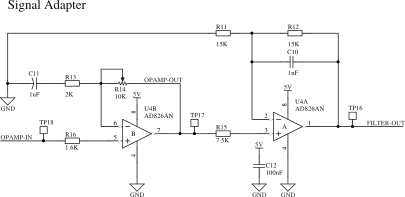
\includegraphics[width=.8\linewidth]{figures/circuits/filter-ampl.pdf}
    \caption[Circuito di adattamento del segnale]{
        Circuito di adattamento del segnale in entrata.
        \label{fig:filter-ampl}
    }
\end{figure}

\`E importante notare che per questa applicazione si \`e scelto utilizzare
degli opamp \emph{rail to rail}, che hanno una tensione di saturazione vicina
a quella di alimentazione. Essi sono necessari per poter raggiungere tensioni
vicino allo 0\,V, che non sarebbero possibili con un opamp normale siccome
l'alimentazione del circuito \`e asimmetrica tra 0 e 12\,V.

\paragraph{Amplificatore.} Come si pu\`o notare a sinistra nella figura
\ref{fig:filter-ampl}, il circuito di amplificazione non ha una configurazione
tipica. Esso \`e basato su una configurazione non invertente ma dispone di un
consensatore (C11) che modifica la retroazione in modo da reagire unicamente
alla componente AC del segnale. Questo permette di amplificare la componente
alternata ignorando l'offset del segnale, perci\`o di \emph{non} utilizzare
un'alimentazione simmetrica \(\pm\)5\,V.

L'amplificazione di questo amplificatore \`e comunque data dal rapporto
\(1+R_{14}/R_{13}\) che permette un un guadagno fino a 6 oppure 15,5\,dB.


\paragraph{Filtro.} A destra della figura \ref{fig:filter-ampl} vi \`e il
circuito di filtraggio, realizzato utilizzando un tipico filtro passa basso
attivo di primo ordine. Esso \`e dimensionato con una frequenza di taglio di
10\,kHz poich\`e quest'ultimo \`e il limite di Nyquist, conosciuto anche dal
teorema di Shannon, il quale stata che la frequenza di campionamento deve
essere almeno doppia della frequenza dell'armonica di frequenza maggiore.

Anche il filtro essendo non invertente ha un rapporto di amplificazione dato
da \(1+R_{12}/R_{11}\). Nella figura il valore della resistenza \(R_{11}\) \`e
\textbf{incorretto} (Vedi sezione \ref{sec:err-filter}). Dopo la correzzione
il filtro ha un amplificazione approssimativamente unitaria.

\section{Microcontroller}

\section{Visualizzazione}

	\chapter{Software}
\section{Campionamento}
\section{Interfaccia al Computer}
\section{Interfaccia al Display}
\section{Fast Fourier Transform}

	\chapter{Conclusioni}
\section{Problemi riscontrati}


\subsection{Errore nella scelta dell'opamp} \label{sec:err-opamp}
\subsection{Errore nel dimensionamento del filtro attivo}
\subsection{Sincronizzazione dei threads}
\lstinputlisting[language=diff]{res/serialworker-crash-fix.diff}

\section{Commento}
\section{Certificazione}
Il sottoscritto dichiara di aver redatto e prodotto individualmente il lavoro
di produzione.
\begin{flushright}
\begin{tabular}{ r p{5cm} p{1cm} r p{5cm}}
    Data: & \hrulefill && Firma: & \hrulefill \\
    &&&& Naoki Pross \\
\end{tabular}
\end{flushright}


    %\appendix
    \chapter{Trasformata di Fourier}

\section{Nozioni preliminarie}

\subsection{Regressione lineare con il metodo dei minimi quadrati}
La regressione lineare \`e un'approssimazione di una serie di dati ad una
funzione lineare. Questa retta di approssimazione pu\`o essere calcolata in
molteplici modi, per questo progetto \`e di interesse utilizzare il
\emph{metodo dei minimi quadrati}.  Sar\`a dunque esplicato come trovare i
coefficienti di una retta a \(m+1\) termini partendo da \(N\) punti di
riferimento.
\begin{equation}
    r(x, a_0, \dots, a_m) = a_0 + x\sum_{i=1}^{m}a_i
\end{equation}
Consideriamo di avere gli insiemi \(X\) e \(Y\) entrambi con \(N\) termini di
cui si prende le coppie ordinate di valori \((x_k, y_k)~ x_k\in X,\,y_k\in
Y\), ossia i punti dato di cui eseguire la regressione.  Il metodo dei minimi
quadrati trova i coefficienti della retta minimizzando il quadrato della
differenza tra il valore stimato dalla retta \(r(x_k)\) e il valore reale
\(y_k\).
\begin{equation*}
    \min((r(x_k) - y_k)^2)\quad \forall x_k\in X,\, y_k\in Y
\end{equation*}
Definiamo quindi la funzione da minimizzare \(\varepsilon\)
\begin{equation}
    \varepsilon(a_0, \dots, a_m) = \sum_{k=1}^{N}\Big[r(x_k, a_0, \dots, a_m)  - y_k\Big]^2
\end{equation}
Da cui si computa le derivati parziali rispetto ai coefficienti ricercati,
ottenendo un sistema di equazioni lineare. Ci\`o corrisponde anche ad
affermare che il \emph{gradiente} di \(\varepsilon\) \`e un vettore
\(\in\mathbb{R}^{m+1}\) con tutte le componenti a 0.
\begin{equation*}
    \nabla\varepsilon = \langle 0, \dots, 0 \rangle
\end{equation*}
A questo punto si pu\`o procedere risolvendo il sistema con l'algebra lineare
definendo la matrice di trasformazione \(\mathbf{A}\) e il vettore dei termini
noti \(\vec{u}\)
\begin{equation*}
    \nabla \varepsilon = \mathbf{A}
        \langle a_0, \dots,  a_m \rangle + \vec{u} \iff
    \langle a_0, \dots, a_m \rangle =
        \mathbf{A}^{-1}(-\vec{u})
\end{equation*}

\subsection{Funzione armonica}
Una funzione armonica, sinusoidale, pu\`o essere descritta in molteplici modi.
Iniziamo dunque osservando le forme pi\`u semplici, ossia la forma
trigonometrica.
\begin{align} \label{eq:harmonics-trig}
    f(x) &= a\cdot\sin (\omega x + \varphi) \\
    f(x) &= b\cdot\cos(\omega x + \vartheta)
\end{align}
Conoscendo la formula di Eulero \eqref{eq:euler}
\begin{equation} \label{eq:euler}
    e^{i\varphi} = \cos(\varphi) + i\cdot\sin(\varphi)
\end{equation}
possiamo riscrivere \(f(x)\) nei seguenti modi
\begin{align} \label{eq:harmonics-complex}
    f(x) &= \frac{a}{2i}\cdot(e^{i(x\omega + \varphi)} - e^{-i(x\omega + \varphi)}) \\
    f(x) &= \frac{b}{2}\cdot(e^{i(x\omega + \vartheta)} + e^{-i(x\omega + \vartheta)})
\end{align}

\subsection{Propriet\`a di ortogonalit\`a del seno e del coseno}
Per avere delle fondamenta solide prima dell'introduzione dell'argomento
principale, saranno dimostrate le propriet\`a di ortogonalit\`a del seno e
coseno. Considerando il periodo \(T\), dunque di frequenza \(2\pi /\,T\).

\paragraph{Intuizione geometrica}

\paragraph{Dimostrzioni algebriche }
\begin{enumerate}
\item {
    \begin{align*}
        \int_0^T \sin(\frac{m2\pi x}{T})\,\dd{x} &= 0
        \quad \forall m \in \mathbb{Z} \\
        %
        \int_0^T \sin(\frac{m2\pi x}{T})\,\dd{x}
        &= \bigg [-\frac{T}{2\pi m }\cdot\cos\big(\frac{2\pi}{T}mx\big)\bigg]^T_0 \\
        &= -\frac{T}{2\pi m}\cdot\cos\big(2\pi m\big) 
            +\frac{T}{2\pi m}\cdot\cos\big(0\big) \\
        &= 0
    \end{align*}
}

\item {
    \begin{align*}
        \int_0^T \cos(\frac{m2\pi x}{T})\,\dd{x} &= 0
        \quad \forall m \in \mathbb{Z}^* \\
        %
        \int_0^T \cos(\frac{m2\pi x}{T})\,\dd{x}
        &= \bigg [\frac{T}{2\pi m}\cdot\sin\big(\frac{2\pi}{T}mx\big)\bigg]^T_0 \\
        &= \frac{T}{2\pi m}\cdot\sin\big(2\pi m\big) 
            +\frac{T}{2\pi m}\cdot\sin\big(0\big) \\
        &= 0
    \end{align*}
    Nota: Se \(m = 0\) 
    \[\int_0^T \cos(\frac{m2\pi x}{T})\,\dd{x} = T\]
}

\item {
}
\end{enumerate}

% \begin{align*}
%     & \int_0^T \sin(\frac{m2\pi x}{T})\,\dd{x} = 0
%         \quad \forall m \in \mathbb{Z} \\
%     %
%     & \int_0^T \cos(\frac{m2\pi x}{T})\,\dd{x} = 0
%         \quad \forall m \in \mathbb{Z^*} \\
%     %
%     & \int_0^T \sin(\frac{m2\pi x}{T})\cos(\frac{n2\pi x}{T})\,\dd{x} = 0
%         \quad \forall m,n \in \mathbb{Z} \\
%     %
%     & \int_0^T \sin(\frac{m2\pi x}{T})\sin(\frac{n2\pi x}{T})\,\dd{x} = 0 
%         \quad \forall m,n \in \mathbb{Z}~|~m\neq \pm n \\
%     %
%     & \int_0^T \sin^2(\frac{m2\pi x}{T})\,\dd{x} = \frac{T}{2}
%         \quad \forall m \in \mathbb{Z} \\
%     %
%     & \int_0^T \cos(\frac{m2\pi x}{T})\cos(\frac{n2\pi x}{T})\,\dd{x} = 0 
%         \quad \forall m,n \in \mathbb{Z}~|~m\neq \pm n \\
%     %
%     & \int_0^T \cos^2(\frac{m2\pi x}{T})\,\dd{x} = \frac{T}{2}
%         \quad \forall m \in \mathbb{Z^*} \\
% \end{align*}

\section{Polinomio Trigonometrico}
Analogamente a come \`e definito un polinomio \(P\) ``normale'' di grado
\(N\), \`e possibile definire anche un polinomio trigonometrico \(T\).
\[
    P_N(x) = \sum_{n=0}^N a_n x^n \qquad a_n \in \mathbb{R},~ a_N \neq 0
\]
\[
    T_N(x) = \sum_{n=0}^N c_n e^{i\omega nx} 
        \qquad c_n \in\mathbb{C},~\omega\in\mathbb{R}, ~ c_N \neq 0
\]
Questo polinomio \`e detto \emph{trigonometrico} perch\`e utilizzando la
formula di eulero \(e^{i\varphi} = \cos(\varphi) + i\sin(\varphi)\) si pu\`o
espandere nel seguente modo.
\[
    T_N(x) = \sum_{n=0}^N\big [a_n\cdot\cos(\omega nx) + ib_n\cdot\sin(\omega nx)]
    \qquad a_n, b_n \in \mathbb{C}
\]
\`E definito inoltre il polinomio trogonometrico \emph{reale} come
\[
    T_N(x) = \sum_{n=0}^N\big [a_n\cdot\cos(\omega nx) + b_n\cdot\sin(\omega nx)]
    \qquad a_n, b_n \in \mathbb{R}
\]
Quest'ultimo mediante delle identit\`a trigonometriche pu\`o essere riscritto
anche nel modo seguente.
\[
    T_N(x) = \sum_{n=0}^N A_n\cdot\cos(\omega nx - \varphi)
\]

In tutti i casi possiamo osservare che il polinomio trogonometrico \`e una
somma di sinusoidi di frequenze multiple ad una base \(\omega = 2\pi f\).
Se descritto mediante la terminologia dell'algebra lineare, si pu\`o anche
osservare che un polinomio trigonometrico \`e una combinazione lineare nello
spazio funzionale ortonormato dalle basi \(\sin(\omega nx)\) e \(\cos(\omega
nx)\).


\section{Serie di Fourier}

\section{Trasformata di Fourier discreta}
La Trasformata di Fouerier Discreta (DFT) \`e l'operazione matematica che
permette di trovare i coefficienti della serie di Fourier o di un polinomio
trigonometrico, per approssimare al meglio una funzione. Se presa a sestante
per\`o essa essendo una \emph{trasformata} pu\`o essere osservata anche come
una funzione che da uno spettro \emph{discreto} di una funzione. La densit\`a
spettrale ottenuta dalla DFT \`e dipende dalla frequenza di base scelta e nel
caso di un polinomio trigonometrico, anche dal numero di termini di
quest'ultimo.
\[
    \hat{f_k} = \frac{1}{T}\int_0^T f(x)\cdot e^{-ik2\pi fx}\,\dd{x}
\]

\subsection{Derivazione della DFT}
Per trovare la DFT, supponiamo di voler approssimare una funzione \(f\),
utilizzando il metodo dei minimi quadrati, con un polinomio trigonometrico
reale.
\[
    T_N(x) =  \sum_{n=0}^N A_n\cdot\cos(\omega nx -\varphi) \qquad \omega=2\pi f
\]
Sappiamo che questo pu\`o essere scritto anche nel seguente modo.
\[
    T_N(x) =  \sum_{n=0}^N a_n\cdot\cos(\omega nx)  + b_n\cdot\sin(\omega nx)
\]

Dunque per trovare i termini \(a_0,\dots,a_N\) e \(b_0,\dots,b_N\) definiamo
una funzione \(\varepsilon\) da minimizzare con il metodo dei minimi quadrati.
\[
    \varepsilon = \int_0^T\big[T_N(x) - f(x)\big]^2\,\dd{x}
\]

Per generalizzare sar\`a dimostrato come trovare il \(k\)-esimo termine.
\[
    \frac{\partial\varepsilon}{\partial a_k} =
    \frac{\partial}{\partial a_k} \int_0^T\big[T_N(x) - f(x)\big]^2\,\dd{x}
    = 0
\]
\[
    \frac{\partial\varepsilon}{\partial b_k} =
    \frac{\partial}{\partial b_k} \int_0^T\big[T_N(x) - f(x)\big]^2\,\dd{x}
    = 0
\]

\subsubsection{Termini dei coseni}
\begin{align*}
    \frac{\partial\varepsilon}{\partial a_k} =
    \frac{\partial}{\partial a_k} \int_0^T\big[T_N(x) - f(x)\big]^2\,\dd{x}
    &= 0 \\
\end{align*}
\subsubsection{Termini dei seni}

\section{Trasformata di Fourier}

\section{Fast Fourier Transform}
\subsection{Motivazioni e Complessit\`a temporale}
\subsection{Propriet\`a dei numeri complessi}



    \begin{thebibliography}{2}
\bibitem{example}
    \textit{Example item title},
    (online), Author and other informations, \\
    \url{https://www.example.com}

\end{thebibliography}


    \afterpage{
        \newgeometry{margin=1.5cm}
        \pagestyle{empty}

        %\chapter*{Allegati}
        \addcontentsline{toc}{chapter}{Allegati}
        \stepcounter{chapter}

        \addcontentsline{toc}{section}{Pianificazione del progetto}
        \includepdf[pages={-}, angle=90]{Pianificazione.pdf}

        \addcontentsline{toc}{section}{Diario giornaliero}
        \includepdf[pages={-}]{journal.pdf}

        \addcontentsline{toc}{section}{Schema Elettrico}
        \includepdf[pages=-, angle=90]{res/schematic.pdf}

        \section*{Codice sorgente}
        \subsection*{Codice del microcontroller}
        \begin{figure}[H] \centering
            \includegraphics{figures/uml/embedded-flowchart}
            \caption{Diagramma di flusso del codice del microcontrollore}
        \end{figure}

        \lstinputlisting{../src/main.c}
        \lstinputlisting{../src/hwconfig.h}

        \subsubsection*{Fast Fourier Transform}
        \lstinputlisting{../src/fft.h}
        \lstinputlisting{../src/fft.c}

        % \subsubsection*{Controllo del display}
        % \lstinputlisting{../src/ht1632.h}
        % \lstinputlisting{../src/ht1632.c}
        
        \subsubsection*{Libreria RS232}
        \lstinputlisting{../src/rs232.h}
        \lstinputlisting{../src/rs232.c}

        \subsection*{Codice dell'applicativo desktop}
        \lstinputlisting[language=c++]{../src-desktop/main.cpp}

        \subsubsection*{Finestra principale}
        \lstinputlisting[language=c++]{../src-desktop/mainwindow.h}
        \lstinputlisting[language=c++]{../src-desktop/mainwindow.cpp}

        \subsubsection*{Gestione della risorsa seriale}
        \lstinputlisting[language=c++]{../src-desktop/serialworker.h}
        \lstinputlisting[language=c++]{../src-desktop/serialworker.cpp}

        \clearpage
        \restoregeometry
    }

\end{document}
